\subsection{Block Diagram}
\begin{center}
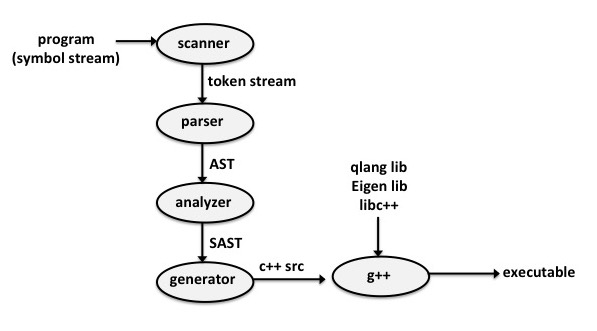
\includegraphics[scale=0.65]{architectural_diagram/architecture.jpg}
\end{center} 
\subsection{Components}
\begin{enumerate}
\item Scanner\\\\
The scanner was implemented using ocamellex - the associated file is scanner.mll. It was chiefly implemented by Christopher Campbell and Winnie Narang.\\\\
The scanner takes a program (symbol stream) as input and tokenizes it to produce a token stream. The tokenization process provides basic syntax checking, rejecting programs that contain illegal symbols and illegal combinations of symbols (e.g. the \$ symbol). Additionally, it discards information that is unnecessary for the remainder of the compilation process such as white space and comments.\\
\item Parser \& Abstract Syntax Tree\\\\
The parser was implemented using ocamlyacc - the associated files are ast.ml and parser.mly. It was chiefly implemented by Christopher Campbell and Sankalpa Khadka.\\\\
The parser takes the token stream produced by the scanner as input and parses it to produce an abstract syntax tree (AST), which describes the overall structure of the program. ast.ml provides parser.mly with the acceptable structure of the AST. The parsing process provides further syntax checking, rejecting programs that do not strictly meet the syntactic requirements of the AST (e.g. a malformed for statement).\\
\item Analyzer \& Semantically Analyzed Syntax Tree\\\\
The analzyer was implemented in OCaml - the associated files are analyzer.ml and sast.ml. Additionally, analyzer.ml utilizes ast.ml in order to be able to analyze its input. It was chiefly implemented by Christopher Campbell.\\\\
The analyzer takes the ast produced by the parser and analyzes it to produce a semantically analyzed abstract syntax tree (SAST). Like the AST, the SAST describes the overall structure of the program, but it also includes type information that was attached during the analysis process. sast.ml provides analyzer.ml with the acceptable structure of the SAST. The analysis process provides rigorous semantic checking, rejecting programs that violate type requirements (e.g. assigning a complex number to a variable declared as an integer), declaration requirements (e.g. using a variable that was not declared or attempting to declare a variable more than once), scope requirements (e.g. using a variable declared in another function), order requirements (e.g. calling a function before it is declared), and other language-specific requirements (e.g. not declaring a compute function). Additionally, the analyzer adds built-in information (i.e. built-in variables and functions) to the sast.\\
\item Generator\\\\
The generator was implemented in OCaml - the associated file is generator.ml. Additionally, generator.ml utilizes sast.ml in order to be able to process its input. It was chiefly implemented by Sankalpa Khadka, Jonathan Wong, and Winnie Narang.\\\\
The generator takes the sast produced by the analyzer and generates c++ code from it. Most of the code it generates is hard coded into generator.ml, but but it also draws on code from our standard library - qlanglib, libc++, and Eigen (a third-party library).\\
\item QLang Library\\\\
The QLang Library was implemented in c++ - the associated files are qlang.hpp and qlang.cpp. It was chiefly implemented by Jonathan Wong. The QLang library contains c++ code for carrying out some of the more complex conversions from qlang code to c++ code in the generator (e.g. generating qubits and carrying out the tensor product).
\end{enumerate}